\section{}
Referring to Figure \ref{fig:Q2ProblemDiagram}, verify the results 
\begin{align*}
    \int_{0}^{\pi/2} (\sigma_r \sin\theta) r d\theta = \int_{0}^{\pi/2} \frac{2P}{\pi} \sin\theta \cos\theta d\theta = \frac{P}{\pi} \\
    \int_{-\pi/2}^{\pi/2} (\sigma_\theta \cos\theta) r d\theta = \int_{-\pi/2}^{\pi/2}\frac{2P}{\pi} \cos^2\theta d\theta = P 
\end{align*}
\begin{figure}[h]
    \centering
    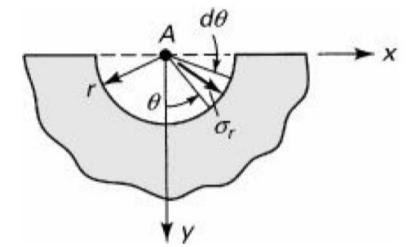
\includegraphics[width=0.35\linewidth]{Questions/Figures/Q2ProblemDiagram.png}
    \caption{Problem diagram for Question 2.}
    \label{fig:Q2ProblemDiagram}
\end{figure}

For radial stress distribution in a very large plate (semi-infinite solid) under normal load at its horizontal surface,
(Eq. 3.48 in the textbook)
\begin{equation*}
    \sigma_r = \frac{2P}{\pi r} \cos\theta
\end{equation*}
Verifying the first integral,
\begin{align*}
    \int_{0}^{\pi/2} (\sigma_r \sin\theta) r d\theta &= \int_{0}^{\pi/2} \frac{2P}{\pi} \sin\theta \cos\theta d\theta \\
    &= \frac{2P}{\pi} \int_{0}^{\pi/2} \sin\theta \cos\theta d\theta \\
    &= \frac{2P}{\pi} \int_{0}^{\pi/2} \frac{1}{2} \sin(2\theta) d\theta \\
    &=\frac{2P}{\pi} \left[-\frac{1}{4} \cos(2\theta) \right]_{0}^{\pi/2} \\
    &= \left(\frac{2P}{\pi}\right) \left[-\left(\frac{1}{4} (-1) - \frac{1}{4} (1) \right)\right] \\
    &= \boxed{\frac{P}{\pi}}
\end{align*}
Verifying the second integral,
\begin{align*}
    \int_{-\pi/2}^{\pi/2} (\sigma_\theta \cos\theta) r d\theta &= \int_{-\pi/2}^{\pi/2}\frac{2P}{\pi} \cos^2\theta d\theta \\
    &= \frac{2P}{\pi} \int_{-\pi/2}^{\pi/2} \frac{1}{2} (1 + \cos(2\theta)) d\theta \\
    &= \frac{P}{\pi} \left[\theta + \frac{1}{2} \sin(2\theta) \right]_{-\pi/2}^{\pi/2} \\
    &= \frac{P}{\pi} \left(\frac{\pi}{2} + \frac{1}{2} (-1) + \frac{\pi}{2} + \frac{1}{2} (1) \right) \\
    &= \frac{P}{\pi} \pi \\
    &= \boxed{P}
\end{align*}